\documentclass[11pt]{article}
\usepackage[utf8]{inputenc}
\usepackage[T1]{fontenc}
\usepackage{graphicx}
\usepackage{grffile}
\usepackage{longtable}
\usepackage{wrapfig}
\usepackage{rotating}
\usepackage[normalem]{ulem}
\usepackage{amsmath}
\usepackage{textcomp}
\usepackage{amssymb}
\usepackage{capt-of}
\usepackage{hyperref}
\usepackage{minted}
\usepackage[section]{placeins}
\author{Student: Brian Cheung bc32427 \\ Professor: Mohit Tiwari \\ TA: Antonio Espinoza \\ Department of Electrical \& Computer Engineering \\ The University of Texas at Austin}
\date{\today}
\title{EE379K Enterprise Network Security Lab 1 Report}
\hypersetup{
 pdfauthor={Student: Brian Cheung bc32427 \\ Professor: Mohit Tiwari \\ TA: Antonio Espinoza \\ Department of Electrical \& Computer Engineering \\ The University of Texas at Austin},
 pdftitle={EE379K Enterprise Network Security Lab 1 Report},
 pdfkeywords={},
 pdfsubject={},
 pdfcreator={},
 pdflang={English}}
\begin{document}

\maketitle
\newpage
\section*{Part 1 - Server and Client Networking}
\label{sec:part-1}
The task was to implement an echo server and client in C given a Python implementation that modeled the desired behavior of the server and client.
The Python implementation was also used to test the compatibility of the C program by interchanging the server and client with a Python server and C client and vice versa.
The next task was to perform a Denial of Service (DOS) attack on the C server.
\subsection*{Step 1 - Echo Server}
\subsubsection*{Build server and client}
In a terminal window, start at root directory of project and run the following commands:
\begin{minted}{bash}
  $ cd Part\ 1
  $ make
\end{minted}
\subsubsection*{Run server and client}
Run the following commands to start the server:
\begin{minted}{bash}
  $ cd Part\ 1
  $ ./server
\end{minted}
Open a new terminal window and run the following commands to start the client:
\begin{minted}{bash}
  $ cd Part\ 1
  $ ./client
\end{minted}
\subsection*{Step 2 - DOS Attack}
The DOS attack was performed using a program called \textbf{\emph{hping3}}.
\noindent The following command was used to perform the DOS attack:
\begin{minted}{bash}
  $ sudo hping3 -S -w 64 -p 12000 --flood --rand-source 127.0.0.2
\end{minted}
\textbf{\emph{hping3}} command flags and options:

\textbf{-S}: flood with SYN packets

\textbf{-p 12000}: specify destination port 12000

\textbf{--flood}: send packets as fast as possible

\textbf{--rand-source}: generates a spoofed IP address to hide the source IP

\textbf{127.0.0.2}: IP address of server
\newline

This command floods the server with SYN packets which tell the server that clients would like to connect.
However, the spoofed IP address prevents the server from sending its SYN-ACK packets back to the correct source IP.
which prevents the three-way handshake from being completed.
Furthermore, this prevents the server from processing other clients' requests because it is too busy trying to complete the attacker's requests,
so actual clients that want to connect to the server are left waiting to complete a three-way handshake until their requests time out.
\newline

The recorded pcap of the attack displays the flood of SYN packets sent to the server (shown in Figure \ref{fig:client-attempt-flood})
along with the server attempting send SYN-ACK packets back to the clients.
However, the server sends the packets to the spoofed IP of the attacker instead,
which prevents the three-way handshake from being completed.
As a result, the client's request times out (shown in Figure \ref{fig:filtered-dos}).

\begin{figure}[h]
\centering
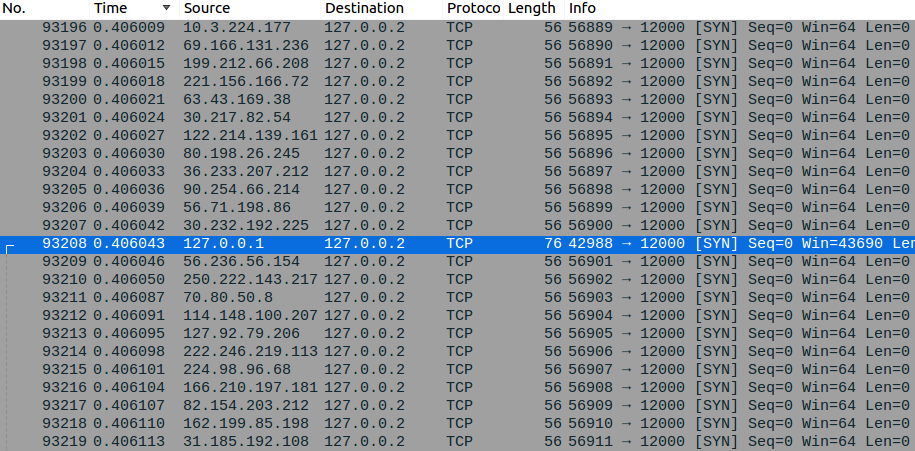
\includegraphics[width=.9\linewidth]{./client-attempt-flood.png}
\caption{\label{fig:client-attempt-flood}
Client with IP address of 127.0.0.1 attempts to connect to the server during a DOS attack.}
\end{figure}

\begin{figure}[h]
\centering
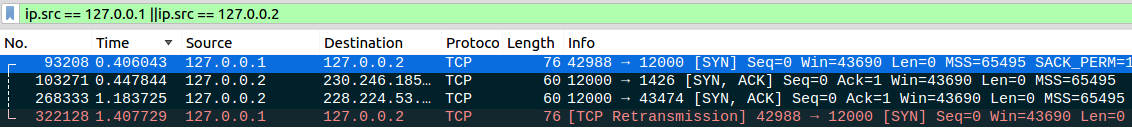
\includegraphics[width=.9\linewidth]{./filtered-dos.png}
\caption{\label{fig:filtered-dos}
The server sends SYN and ACK packets to the spoofed IP of the attacker and the client's request times out.}
\end{figure}

\newpage
\section*{Part 2 - Scan the Internet}
\label{sec:part-2}
The objective of this part was to scan the internet with zmap and group IP addresses in the same network.
\subsection*{ZMAP scan}
The first step required a 2-4 hour zmap scan in order to obtain a list of IP addresses that responded when probed.
\newline

\noindent The following command was used to perform the zmap scan for three hours:
\begin{minted}{bash}
  $ sudo zmap \
      --bandwidth=1M \
      --target-port=80 \
      --blacklist-file=blacklist.txt \
      --output-file=zmap_scan.csv \
      -t 10800
\end{minted}
ZMAP scan results:

\textbf{Total number of machines probed}: 16,063,066

\textbf{Number of machines that responded}: 11,448

\textbf{Hitrate}: 0.071\%
\newline

The next task was to group together all of the IP addresses that belong in the same network.
Each network has a range of IP addresses that are defined by the network's Classless Inter-Domain Routing (CIDR).
The whois command was used to obtain the CIDR that each IP address belonged in, however,
some whois outputs have different fields that define the CIDR (CIDR, inetnum, and IPv4 Address), which further complicated the parsing process.
With 11,448 IP addresses, this task was automated with a Python script (Part 2/scan/scan\_networks.py) that kept track of the IP addresses that successfully or unsuccessfully returned the desired network information.
The Python script ran a Bash script (Part 2/scan/whois\_scan.sh) in a 'subprocess' in order to obtain the desired network information from each IP address.
The output of these scripts is contained in the whois\_output.txt file (Part 2/scan/results/whois\_output.txt).

After scanning and collecting all of the desired data, the next step was to group and count the IP addresses in each network.
This task was also automated using a python script (Part 2/analyze/analyze\_networks.py).
The outputs of this script is contained in the directory: Part 2/analyze/results.
\newline

\noindent Description of each output file:
\begin{itemize}
\item\textbf{networks.json}: Dictionary of all networks. Key: Network CIDRs; Value: Number of IP addresses in network

\item\textbf{network\_ip.json}: Dictionary of networks and all IP addresses within each network. Key: Network CIDRs; Value: List of all IP addresses in network

\item\textbf{multiple\_cidrs.json}: List of networks with large IP ranges that cause it to have multiple CIDRs.

\item\textbf{subnets.json}: List of networks where each CIDR is a subnetword of another CIDR in the string.
\end{itemize}

\noindent Observations:
\begin{itemize}
  \item Large networks may need multiple CIDRs in order to represent its IP range.
  \item Some IP addresses returned multiple lines of CIDR fields. This meant that the IP addresses were contained in a subnetwork within a larger network.
\end{itemize}

\newpage
\section*{Part 3 - Connection Modes}
\label{sec:part-3}
For this part, \verb|tcpdump| was used to record the network traffic when accessing 10 websites each over a 10 second time period for each connection mode (Firefox, TOR, VPN).
Then each of the resulting \verb|.pcap| file was analyzed for the average number of packets (shown in Figure \ref{fig:avg-number-packets})
and average packet size (shown in Figure \ref{fig:avg-packet-size}).

\begin{figure}[h]
  \centering
  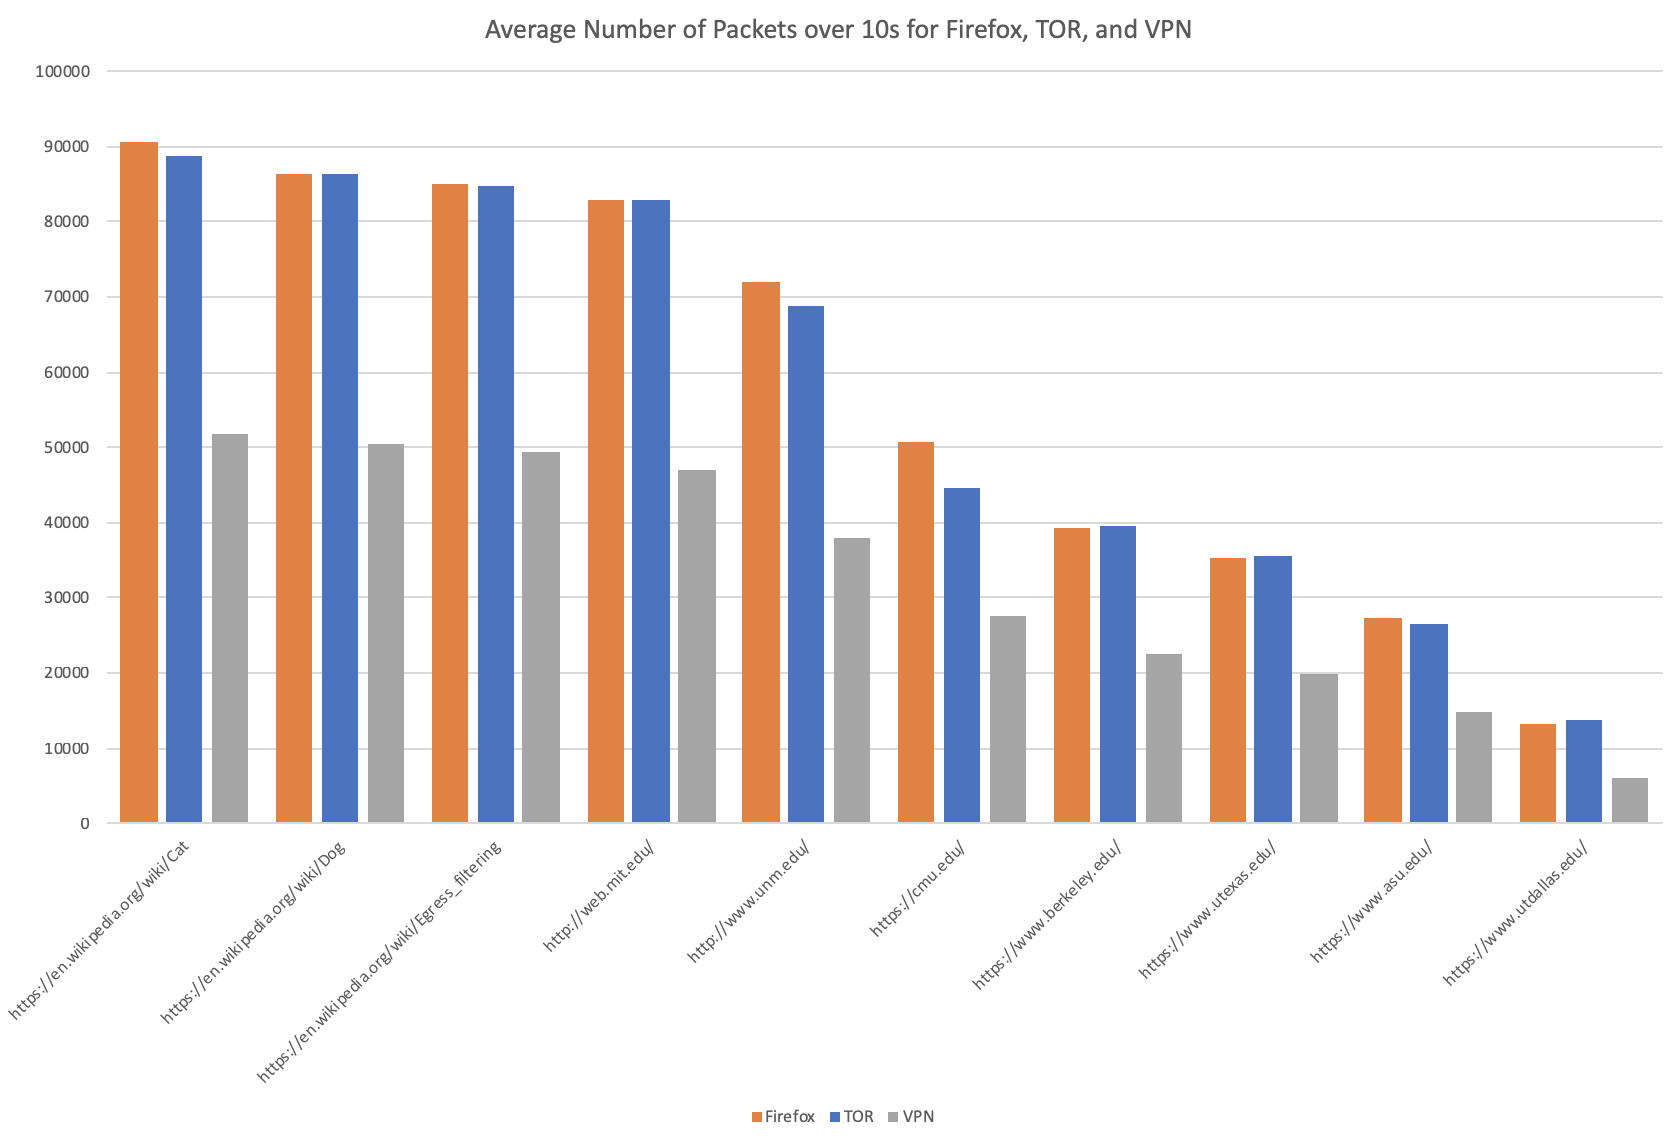
\includegraphics[width=.9\linewidth]{./avg-number-packets.png}
  \caption{\label{fig:avg-number-packets}
  The chart depicts the average number of packets over 10 seconds for each website using each of the 3 connection modes.}
\end{figure}

\begin{figure}[h]
  \centering
  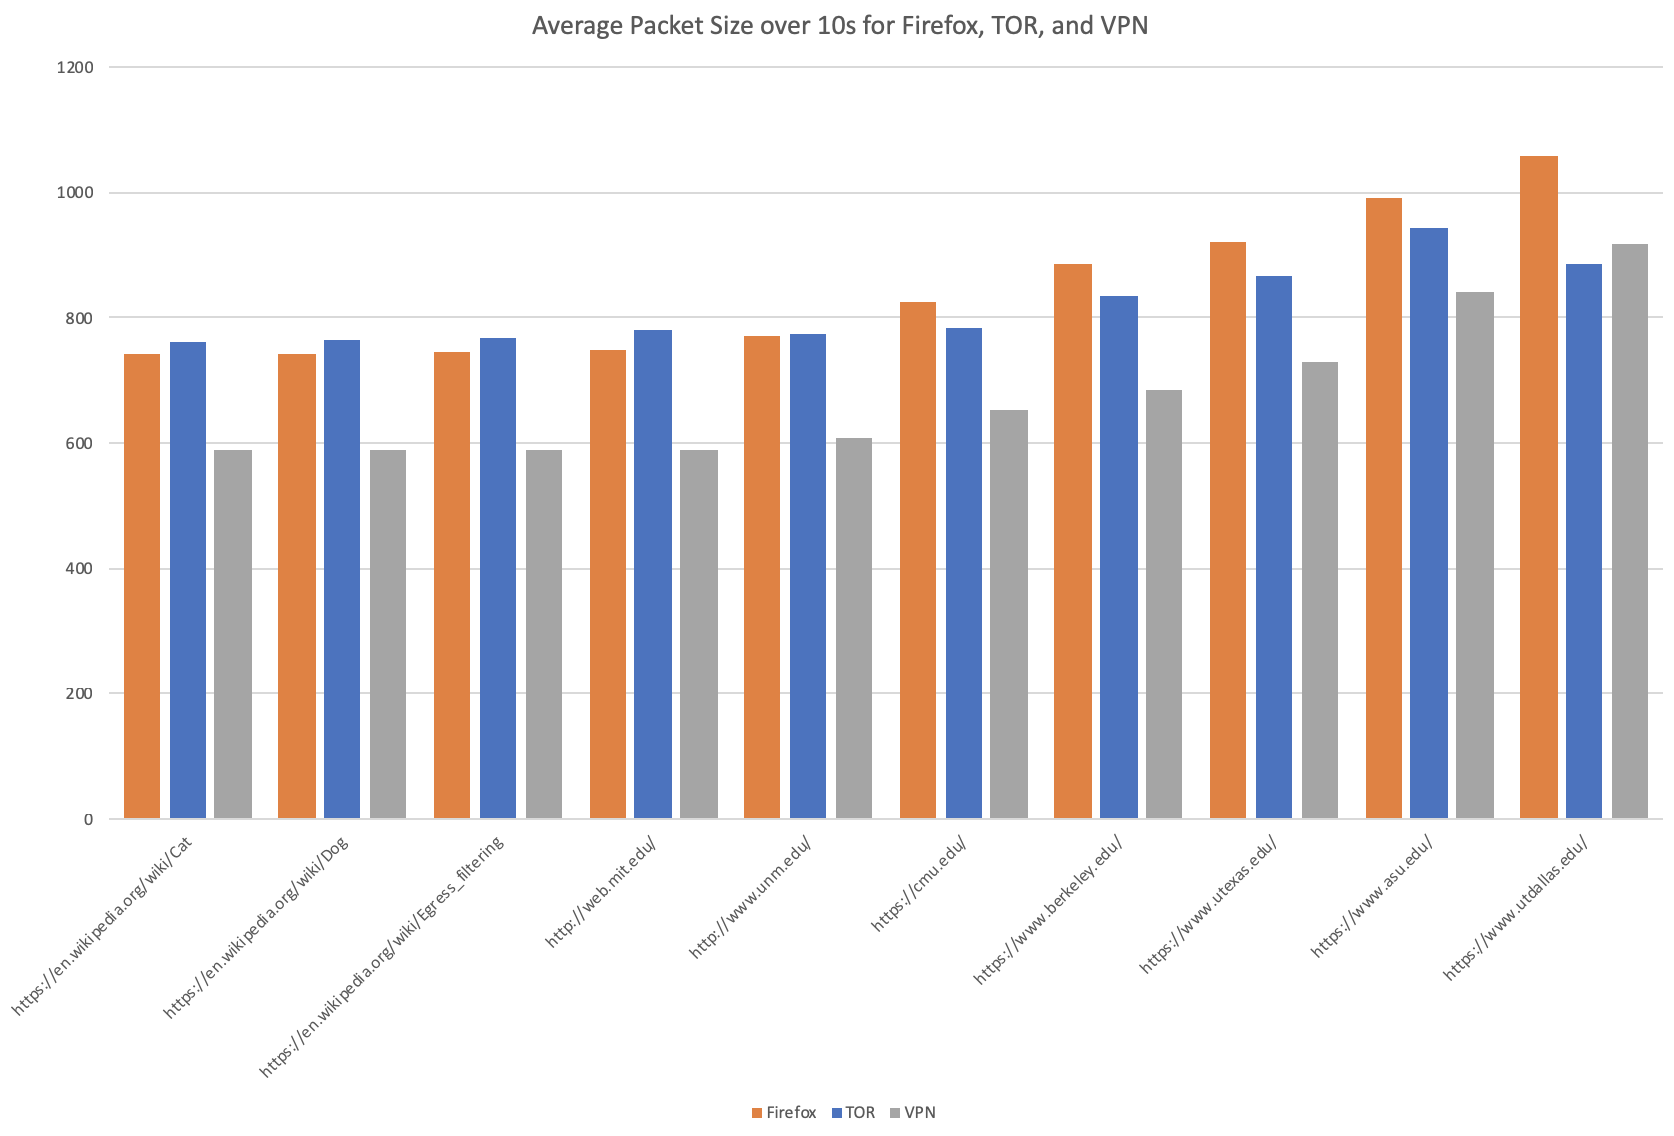
\includegraphics[width=.9\linewidth]{./avg-packet-size.png}
  \caption{\label{fig:avg-packet-size}
  The chart depicts the average packet size over 10 seconds for each website using each of the 3 connection modes.}
\end{figure}

\noindent Observations:
\begin{itemize}
    \item Across every website, and every connection type, the number of pakets sent seemed to decrease with each visit to the same website.
    \item There seems to be an inverse relationship between the number of packets sent and the size of each packet.
    As the average number of packets decreased, the average size of the packets increased.
\end{itemize}

Questions:
\begin{enumerate}
  \item For each connection type, what is visible to a passive device on the network?

  Using a regular browser like Firefox without a VPN or proxy would allow a passive device on the network to
  see which websites were visited as well as the sizes of the packets. With a VPN, a passive device can
  observe the client sending and receiving packets from the VPN server including information about the packet source and destination.
  Lastly, using TOR made it difficult for a passive device to observe which websites were visited.
  The recorded network traffic showed mostly packets being sent to and from \verb|127.0.0.1|
  instead of the IP address of the websites visited.

  \item Can you use the connection statistics to determine which of the 10 websites was visited?

  With the connection statistics from the 10 websites, it may be possible to determine which websites were visited
  because some websites like \verb|wikipedia.org| consistently send smaller packets while transmitting a larger amount.
  This characteristic seemed to persist between all of the \verb|wikipedia.org| websites, which could show that they belong to a similar network.
  Additionally, connection statistics of a video or stream would show a consistent rate packets sent and a consistent packet
  size, which could be easy to identify if one were looking for this characteristic.
\end{enumerate}

\newpage
\section*{Part 4}
\label{sec:part-4}


\section*{Conclusion}
\label{sec:conclusion}
Please provide feedback so we can improve the labs for the course. How many
hours did the lab take you? Was this lab boring? Did you learn anything? Is
there anything you would change? Feel free to put anything here, but leaving it
blank will result in the loss of points.

\nocite{*}
\bibliography{bibliography}
\bibliographystyle{ieeetr}
\end{document}
